\begin{figure}
    \centering
    \includegraphics[width = \linewidth]{src/imgs/visualization-tool.pdf}
    \caption{Source: elaborated by author. The interface of the visualization tool was implemented for the demonstration of use.}
    \label{fig:visualization-tool}
\end{figure}

\section{Visualization tool}
\label{sec:visualization-tool}
A visualization tool was implemented to demonstrate the applicability of the proposed visualization.
%
It was developed a web interface using JavaScript for interactivity and the library D3 for creating plots, the backend of the application was created with the programming language Python and the library Flask.
%

The goals with this tool were to be able to utilize the use case dataset, the proposed plot should be generated in a fast running time to the tool be practical,
%
and furthermore, it was interesting the addition of options and interactivity to increase the analytic capability of the method.

The interface can be visualized in Figure~\ref{fig:visualization-tool}, it can be divided into four panels: the control panel on the top left, the parallel coordinates plot on the top right, the Events-Vis plot in the bottom left and the map view on the bottom right.
%
Each of these panels will be detailed in the following sections.

The user initially selects the dataset on the menu at a), this selection is necessary for the other panels to work.
%
On the control panel, there are options for the generation of the visualization,
%
it is possible to define the projection method used and the optimization method used for the vertical positioning.
%
There are also options that affect the final result of the plot, it is possible to select the color scale for the events and select the option to apply changes in the time scale that will be explained in the following section.

The main view with the Events-Vis Plot is the most important panel, it contains the result of the proposed method. 
%
It is the scatter plot of rectangles, each one representing an event, colored by the attribute selected on the control panel, that can be a numerical or categorical scale.
%

To generate a better visualization, it was considered the development of methods to highlight the regions of the plot where there is more information, i.e., a bigger number of events.
%
Based on the work of~\cite{Janetzko2013} to increase the visibility of the scatter plot, it was included in our plot the distortion of scales.
%
In the time distortion, the time is divided into intervals of the same length, each one will have its width represented in the plot changed to be proportional to the number of events inside the interval.
%
So when an interval is empty, it will be removed from the plot.
%
In Fig.~\ref{fig:time-scale-explanation} is possible to view this time interval, they are marked with vertical grid lines, on the view of the distortion, it is possible to see a highlight on the days at the end of the observed period.
%

After applying this distortion, there is also possible another change that is to, instead of representing events with their original width, make them fit the grid of time intervals.
%
For example, with a time interval of 24h, every event with less than this interval of duration will be plotted with the width if it lasted 24 hours.
%
The use of this modification is to deal with situations where the completed observed time is too big, for example, 30 days, and have events of only a few hours of duration, that will not be shown in the plot.
%
It is a trade-off between the detail in the time information and the visibility of events.
%
Although, our visualization does not support representing the inner structures when events are fit to the grid.
%
A comparison with the three different situations is available in Figure~\ref{fig:time-scale-explanation}.

\begin{figure}
    \centering
    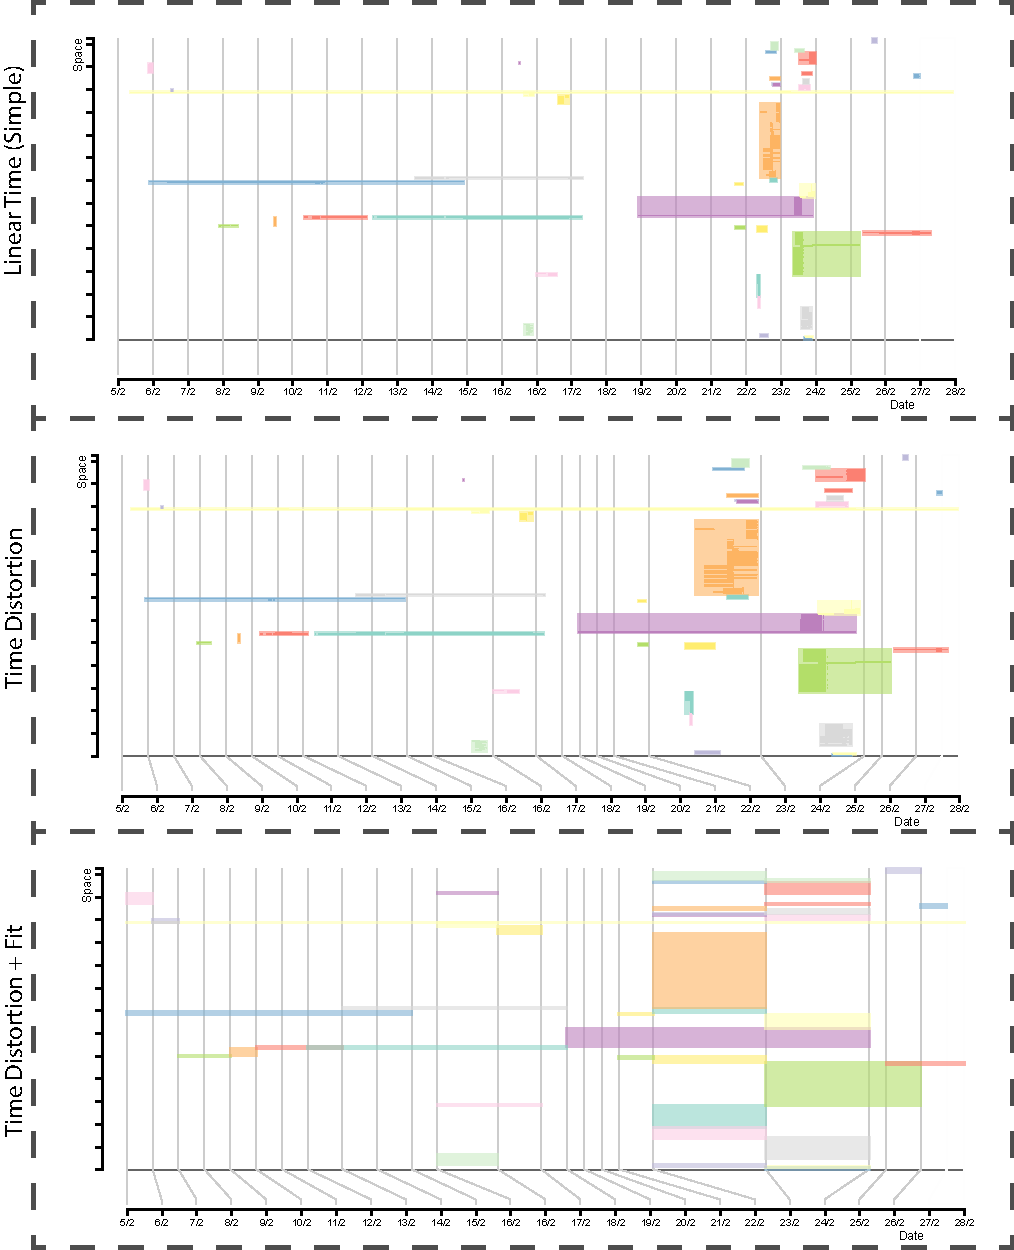
\includegraphics[width = 0.6\textwidth]{src/imgs/time-scale-explanation.pdf}
    \caption{Source: elaborated by author. Comparison of three different types of time scale used in example data from the use case.}
    \label{fig:time-scale-explanation}
\end{figure}

On the left of the plot, there is a color bar that indicates visually the quality of the spatial representation in the y-direction. 
%
This color bar is created by moving all the inner rectangles to the left of the figure, keeping the vertical positions.
%
The color of rectangles is based on a 2D color map from the original space of objects to the vertical position.
%
Each rectangle receives a color based on the center position of the respective point by placing this center position in a grid of size $512\times 512$, and picking the color of the respective pixel in the image of the color map.
%
It is exemplified in Figure~\ref{fig:colormap-example}, with some points in the center of the city of Rio de Janeiro and a respective color bar created.
%
As neighborhoods in the original space will receive similar colors, the continuity of the colors on the bar indicates good neighborhood preservation.

\begin{figure}
    \centering
    \includegraphics[width = 0.6\linewidth]{src/imgs/colormap-example.pdf}
    \caption{Source: elaborated by author. Example of the use of the color map to create a color bar.}
    \label{fig:colormap-example}
\end{figure}

To permit the analysis of different subsets of data and the interpretation of the results of the main plot, two methods for interactivity are implemented that link the Events-Vis view to the other two views.
%

A parallel coordinates plot positioned on the top right of the page is created to permit filtering the data. 
%
The plot contains vertical axes, each based on an attribute. 
%
For each point of data, in our case for each event, a line is placed connecting the positions of the respective values in each scale.
%
In Figure~\ref{fig:parallel-example}, the plot is created based on three attributes of the events: \textit{number of alerts, duration}, and \textit{area}.

\begin{figure}[hb]
    \centering
    \includegraphics[width = 0.7\linewidth]{src/imgs/parallel-coordinates.pdf}
    \caption{Source: elaborated by author. Example of a parallel coordinates with three attributes.}
    \label{fig:parallel-example}
\end{figure}

This permits the user to look for a general overview of the non spatio-temporal attributes,
%
and it is possible to make a selection in each of the axes, filtering the data based on thresholds of these attributes.
%
This filtered data is then pre-processed and the visualization in the main panel is updated, 
%
it permits to avoid cluttering
%
and to analyze spatio-temporal characteristics of objects with properties of particular interest.

On the bottom right of the page, there is a static map that contains a scatter plot of all objects of a particular time interval, a conventional method for the visualization of spatio-temporal data.
%
This data plot is used with selections in the Events-Vis plot, 
%
the users can click in a rectangle to highlight it on the map view.
%
In this map view, the user can look for the individual points by hovering, with a panel with attributes appearing.
